%%%%%%%%%%%%%%%%%%%%%%%%%%%%%%%%%%%%%%%%%%%%%%%%%%%%%%%%%%%%%%%%%%%%%%%%%%%%%%%%
%%% Results
%%%%%%%%%%%%%%%%%%%%%%%%%%%%%%%%%%%%%%%%%%%%%%%%%%%%%%%%%%%%%%%%%%%%%%%%%%%%%%%%

\clearpage
\section{Discussion}
\label{sec:discussion}

\subsection{Results}

%T\"ass\"a osassa esitet\"a\"an tulokset ja vastataan tutkielman alussa
%esitettyihin tutkimuskysymyksiin. Tieteellisen kirjoitelman
%arvo mitataan t\"ass\"a osassa esitettyjen tulosten perusteella.

\nyi{Graphs generated by the system (pictures!)}

% conforming to the JSON graphs (visually?)

\begin{figure}[htb]
\centering 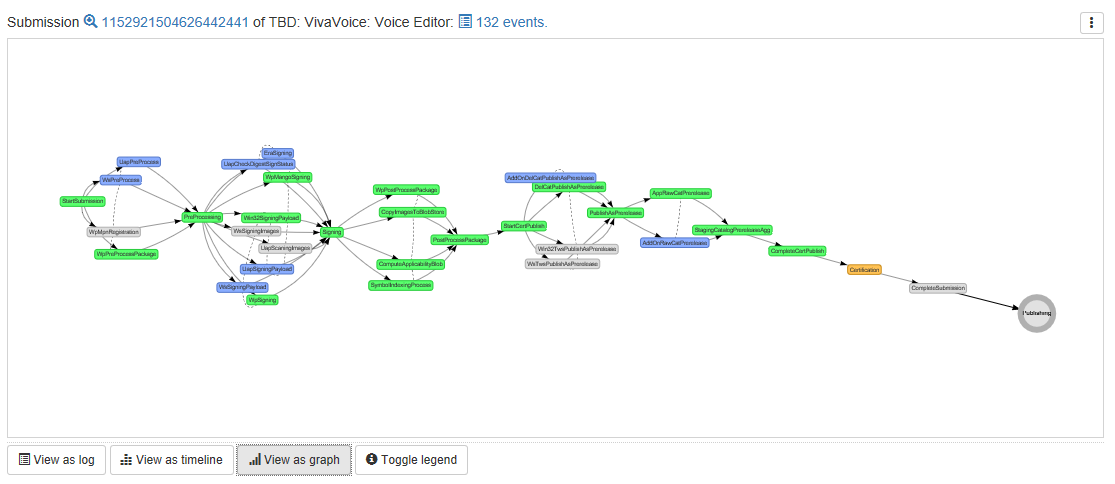
\includegraphics[width=\linewidth]{gfx/graph.png}
\caption{Graph view \label{fig:graph}}
\end{figure}

\begin{figure}[htb]
\centering 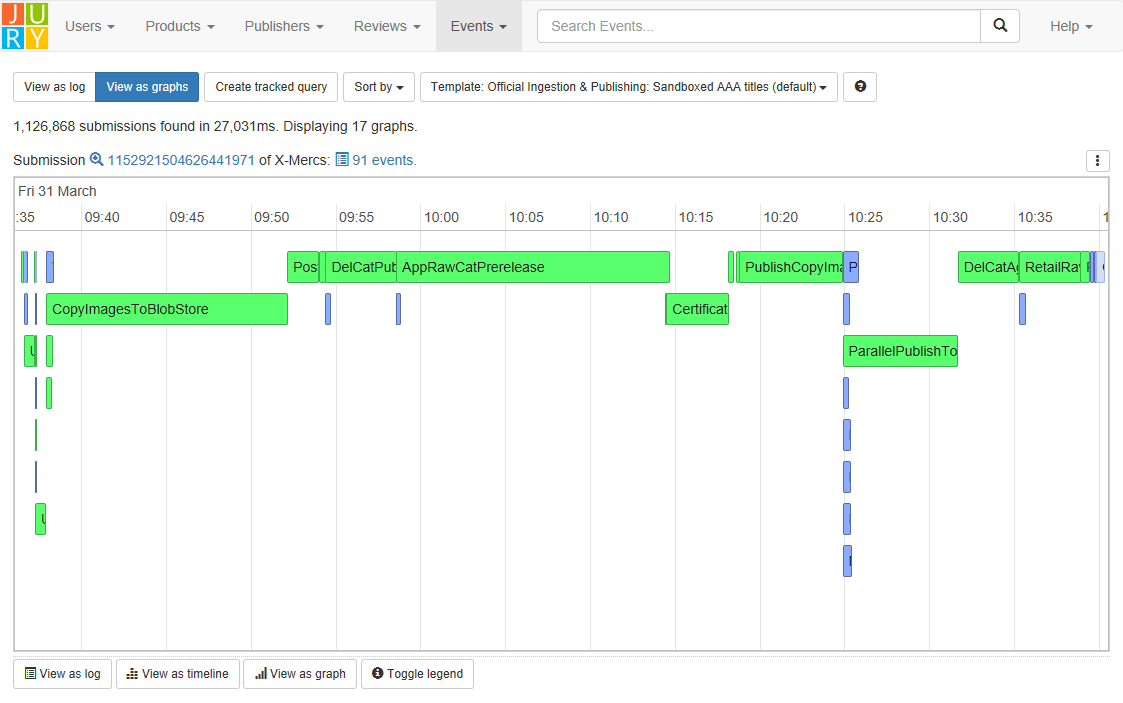
\includegraphics[width=\linewidth]{gfx/timeline.png}
\caption{Timeline view \label{fig:timeline}}
\end{figure}

\begin{figure}[htb]
\centering 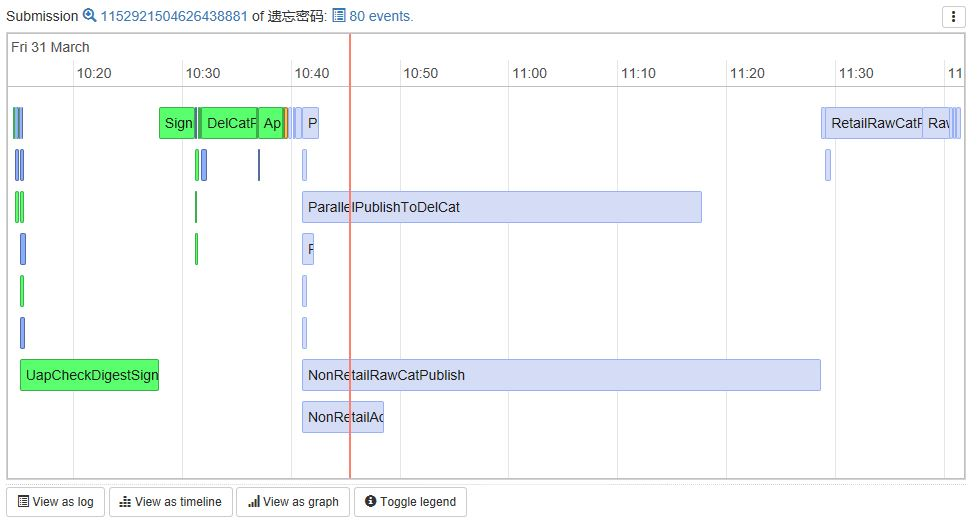
\includegraphics[width=\linewidth]{gfx/estimates.jpg}
\caption{Timeline view with estimates \label{fig:estimates}}
\end{figure}

\nyi{Statistics and their scores}
% (run stats on the same dataset)

\nyi{ML models and their scores}

\begin{table}[htb]
\begin{center}
\begin{tabularx}{\linewidth}{| X | r | r | r | r |}
\hline
~ & \multicolumn{2}{c|}{BDT} & \multicolumn{2}{c|}{Poisson} \\
Dataset & Absolute & RMSE & Absolute & RMSE \\
\hline
\textbf{JSON template} &  &  &  &  \\
No extra features                   & 809.1 & 6290.7 & 881.1 & 5970.6 \\
with current time                   & 825.2 & 6130.3 & 881.1 & 5971.0 \\
with manual review                  & 689.7 & 5819.0 & 809.3 & 5800.9 \\
with resubmission                   & 831.5 & 6255.3 & 881.1 & 5971.2 \\
with manual review and resubmission & 703.7 & 5807.5 & 808.9 & 5800.8 \\
with all extra features             & 693.5 & 5801.9 & 808.3 & 5800.4 \\
\hline
\textbf{Automatically generated template} &  &  &  &  \\
No extra features                   & 994.8 & 5756.3 & 1243.9 & 6563.3 \\
with current time                   & 1099.7 & 6470.5 & 1225.8 & 6558.7 \\
with manual review                  & 815.1 & 5332.1 & 1038.5 & 5785.0 \\
with resubmission                   & 1004.3 & 5845.3 & 1219.1 & 6553.8 \\
with manual review and resubmission & 806.5 & 5428.4 & 1038.4 & 5785.7 \\
with all extra features             & 787.8 & 5234.4 & 1038.6 & 5785.4 \\
\hline
\end{tabularx}
\end{center}
\label{tab:mlresults}
\caption{Results from the best ML models}
\end{table}

\nyi{User satisfaction}

\subsection{Evaluation}
\label{sec:evaluation}

%Tutkimustuloksien merkityst\"a on aina syyt\"a arvioida ja tarkastella
%kriittisesti.  Joskus tarkastelu voi olla t\"ass\"a osassa, mutta se
%voidaan my\"os j\"att\"a\"a viimeiseen osaan, jolloin viimeisen osan nimeksi
%tulee >>Tarkastelu>>. Tutkimustulosten merkityst\"a voi arvioida my\"os
%>>Johtop\"a\"at\"okset>>-otsikon alla viimeisess\"a osassa. 

%T\"ass\"a osassa on syyt\"a my\"os arvioida tutkimustulosten luotettavuutta.
%Jos tutkimustulosten merkityst\"a arvioidaan >>Tarkastelu>>-osassa,
%voi luotettavuuden arviointi olla my\"os siell\"a. 

\nyi{Talk about success with graph generation}\\
\nyi{Maybe talk about alternative graph?}\\
\nyi{Changes in the system reflected real time (also a strength?)}\\
\nyi{Finding bugs in system (race conditions!) based on graphs}\\
\nyi{Feedback from users}

\nyi{Talk about negatives with machine learning models}\\
\nyi{Reason why they didn't end up working}

\nyi{Talk about how the system went immediately into production}\\
\nyi{Talk about the success of notifications built on top of the system}

%%%%%%%%%%%%%%%%%%%%%%%%%%%%%%%%%%%%%%%%%%%%%%%%%%%%%%%%%%%%%%%%%%%%%%%%%%%%%%%%

\subsection{Conclusions and Future Work} 
\label{sec:conclusions}

\begin{itemize}
\item[--]\nyi{Contributions (positives)}
\item[--]\nyi{Limitations (negatives)}
\item[--]\nyi{Future work}
\end{itemize}